\documentclass[
    iai, % Saisir le nom de l'institut rattaché
    il, % Saisir le nom de l'orientation
    %confidential, % Décommentez si le travail est confidentiel
]{heig-tb}

\usepackage[nooldvoltagedirection,european,americaninductors]{circuitikz}
\usepackage{tabularx}
\usepackage{multicol}
\usepackage{graphicx}

\signature{signature_alec_berney.svg}

\makenomenclature
\makenoidxglossaries
\makeindex

\addbibresource{bibliography.bib}

\input{nomenclature}
\input{acronyms}
\newglossaryentry{heig-vd}{
    name=HEIG-VD,
    description={Haute École d'Ingénierie et de Gestion du canton de Vaud}
}
\newglossaryentry{hes-so}{
    name=HES-SO,
    description={Haute École Supérieure de Suisse Occidentale}
}
\newglossaryentry{latex}{
    name=latex,
    description={Un langage et un système de composition de documents}
}
\newglossaryentry{maths}{
    name=mathematics,
    description={Les mathematiques sont ce que les mathématiciens fonts}
}
\newglossaryentry{docker}{
    name=Docker,
    description={Docker est un outil permettant de gérer des containers, une sorte de machine virtuelle plus légère ayant pour but d'encapsuler une ou plusieurs applications / outils technologiques ainsi que toutes les dépendances que ces dernières exigent pour leur bon fonctionnement}
}
\newglossaryentry{kubernetes}{
    name=Kubernetes,
    description={Kubernetes est un système open-source permettant d'automatiser le déploiement, la mise à l'échelle et la gestion des applications conteneurisées}
}
\newglossaryentry{devops}{
    name=DevOps,
    description={Défini tout le processus conteant l'intégration continue, le déploiement continu et la livraison continue}
}
\newglossaryentry{ci}{
    name=CI,
    description={Continuous Integration / Intégration continue}
}
\newglossaryentry{cd}{
    name=CD,
    description={Continuous Deployement / Déploiement continu}
}
\newglossaryentry{github}{
    name=Github,
    description={GitHub is a website and cloud-based service that helps developers store and manage their code, as well as track and control changes to their code}
}
\newglossaryentry{gitlab}{
    name=Gitlab,
    description={GitLab is The DevOps Platform, delivered as a single application. This makes GitLab unique and creates a streamlined software workflow, unlocking your organization from the constraints of a pieced together toolchain}
}
\newglossaryentry{sgbd}{
    name=SGBD,
    description={Système de Gestion de Base de Données (DBMS), logiciel système servant à stocker, à manipuler ou gérer, et à partager des données dans une base de données}
}
\newglossaryentry{mysql}{
    name=MySQL,
    description={Système de gestion de bases de données relationnelles (SGBDR)}
}
\newglossaryentry{fablab}{
    name=Fablab,
    description={Laboratoire permettant tout type de travaux situé à la HEIG-VD }
}
\newglossaryentry{teams}{
    name=Microsoft Teams,
    description={Plateforme collaborative de visioconférence appartenant à Microsoft}
}
\newglossaryentry{backend}{
    name=Backend,
    description={Terme désignant un étage de sortie d'un logiciel devant produire un résultat. On l'oppose au front-end (aussi appelé un frontal) qui lui est la partie visible de l'iceberg}
}
\newglossaryentry{frontend}{
    name=Frontend,
    description={Partie frontale du projet affichant l'interface utilisateur permettant d'utiliser la logique du backen}
}
\newglossaryentry{bd}{
    name=BD,
    description={Une base de données permet de stocker et de retrouver des données structurées, semi-structurées ou des données brutes ou de l'information, souvent en rapport avec un thème ou une activité. Celles-ci peuvent être de natures différentes et plus ou moins reliées entre elles}
}
\newglossaryentry{rest}{
    name=REST,
    description={REST (representational state transfer) est un style d'architecture logicielle définissant un ensemble de contraintes à utiliser pour créer des services web}
}
\newglossaryentry{api}{
    name=API,
    description={Une interface de programmation d’applications ou interface de programmation applicative (souvent désignée par le terme API pour Application Programming Interface) est un ensemble normalisé de classes, de méthodes, de fonctions et de constantes qui sert de façade par laquelle un logiciel offre des services à d'autres logiciels}
}
\newglossaryentry{framework}{
    name=Framework,
    description={En programmation informatique, un framework est un ensemble cohérent de composants logiciels structurels qui sert à créer les fondations ainsi que les grandes lignes de tout ou partie d'un logiciel, c'est-à-dire une architecture}
}
\newglossaryentry{php}{
    name=PHP,
    description={Language de programmation web}
}
\newglossaryentry{laravel}{
    name=Laravel,
    description={Framework web utilisant le language de programmation php}
}
\newglossaryentry{template}{
    name=Template,
    description={Modèle de projet web frontend définissant déjà toute l'interface graphique et étant adaptable au besoin}
}
\newglossaryentry{javascript}{
    name=JavaScript,
    description={Language de programmation web}
}
\newglossaryentry{vuejs}{
    name=Vue.js,
    description={Framework web frontend utilisant le language de programmation Javascript}
}
\newglossaryentry{nodejs}{
    name=Node.js,
    description={Environnement d’exécution JavaScript construit sur le moteur JavaScript V8}
}
\newglossaryentry{ide}{
    name=IDE,
    description={Un environnement de développement est un ensemble d'outils qui permet d'augmenter la productivité des programmeurs qui développent des logiciels}
}
\newglossaryentry{os}{
    name=OS,
    description={En informatique, un système d'exploitation (souvent appelé OS — de l'anglais Operating System) est un ensemble de programmes qui dirige l'utilisation des ressources d'un ordinateur par des logiciels applicatifs}
}
\newglossaryentry{conteneur}{
    name=conteneur,
    description={Un conteneur est une sorte de machine virtuelle allégée contenant une application}
}

\newglossaryentry{tcp}{
    name=TCP,
    description={Transmission Control Protocol, abrégé TCP, est un protocole de transport fiable, en mode connecté, documenté dans la RFC 7931 de l’IETF}
}
% Auteur du document (étudiant-e) en projet de Bachelor
\author{Alec Berney}

% Activer l'option pour l'accord du féminin dans le texte
\genre{male}

% Titre de votre travail de Bachelor
\title{Gestionnaire de travaux du FabLab}

% Le sous titre est optionnel
\subtitle{Travail de Bachelor}

% Nom du professeur responsable
\teacher {Prof. Y. Chevallier (HEIG-VD)}

% Mettre à jour avec la date de rendu du travail
\date{\today}

% Numéro de TB
\thesis{7212}



\surroundwithmdframed{minted}

%% Début du document
\begin{document}
\selectlanguage{french}
\maketitle
\frontmatter
\clearemptydoublepage

%% Requis par les dispositions générales des travaux de Bachelor
\preamble
\authentification

%% Résumé / Version abbrégée
\begin{abstract}
    % Francais
Le Fablab est un laboratoire de la Haute école d'ingénierie et de gestion du canton de Vaud.
Les étudiants peuvent y réaliser toutes sortes de travaux à l'aide de machines ou outils spécifiques. Généralement, ces travaux sont demandés par les étudiants auprès de techniciens.
La gestion de ces demandes ne convient pas aux responsables du Fablab. C'est pourquoi une plateforme web dédiée à la gestion de ces demandes a déjà fait l'objet d'un précédent travail de Bachelor.
Cependant, l'application n'est pas complètement terminée et déployé. C'est pourquoi un nouveau travail de Bachelor a été proposé afin d'améliorer et de compléter ce travail.\\
La plateforme web finale permettra une meilleure gestion des échanges et commandes.\\
Cela aménera également une nouvelle dimension au niveau du suivi et de l'administration du laboratoire.\\
Une procédure claire, allant de la demande à la réalisation du travail demandé, sera également mise en place grâce à cette application.\\
Pour faciliter le suivi des demandes client, la plateforme mettra en place un système de notifications par email et sur l'application elle-même.\\
L'outil web étant à destination des utilisateurs de l'école, l'authentification via un compte de l'école sera fournie.\\

\asterism

% English
The Fablab is a laboratory of the High School of Engineering and Management of the canton of Vaud.
Here, students can carry out all kinds of work with the help of machines, devices or tools that are made available to them. Generally, these works are requested by the students to some technicians.
The management of these requests does not suit the Fablab managers.
This is why a web platform dedicated to the management of these requests has already been the subject of a previous Bachelor work. However, the application is not fully completed and deployed. Therefore, this Bachelor work has been proposed to improve and complete the work. \\
The final web platform allows a better management of exchanges and orders.
It also brings a new dimension to the follow-up and administration of the laboratory.
A clear procedure, from the request to the completion of the work, will also be put in place into this application. \\
To facilitate the follow-up of the customers' requests, the platform implements a notification system by email and on the application itself. \\
As the web tool is intended to reach school users, an authentication with school account will be provided.
\end{abstract}

%% Sommaire et tables
\clearemptydoublepage
{
    \tableofcontents
    \let\cleardoublepage\clearpage
    \listoffigures
    \let\cleardoublepage\clearpage
    \listoftables
    \let\cleardoublepage\clearpage
    \listoflistings
}

\printnomenclature
\clearemptydoublepage
\pagenumbering{arabic}

%% Contenu
\mainmatter

\chapter{Introduction}
L'introduction est une section requise dans un rapport technique. Introduisez votre travail, l'idée de départ et les objectifs attendus. Un lecteur qui découvrirait votre projet au travers de cette introduction devrait ainsi être capable d'en comprendre le cadre, l'idée générale et les aboutissants du projet.

\section{Contexte}
Le FabLab est un laboratoire permettant de réaliser des travaux sur des machines de ce dernier. Actuellement, pour réaliser un travail sur une machine, il est nécessaire de réaliser une demande par email à l'un des techniciens ayant le droit d'usiner sur la machine souhaitée. Une fois la demande reçue, le technicien usine dès qu'il le peut et doit recontacter le mandataire pour lui donner son travail fini. Durant toute cette période, aucun retour n'a été donné au mandataire. En cas de problème avec un travail, le technicien doit également recontacter le client.
Certains défauts majeurs peuvent être identifier avec la procédure actuelle, les voici :
\begin{itemize}
    \item Il n'y a aucun suivi des travaux pour le mandataire, \cite{lieberherr}
    \item Les échanges liés aux travaux peuvent être réalisé via plusieurs canaux (email, Teams, vocal, etc.), \cite{lieberherr}
    \item Risque de désorganisation, \cite{lieberherr}
    \item Manque de clarté quant à la procédure, \cite{lieberherr}
    \item Aucun historique des travaux réalisé,
    \item Gestion problèmes survenus lors du travail compliqué.
\end{itemize}
Une première partie du projet a déjà été réalisée lors du travail de Bachelor de monsieur Tristan Lieberherr. De ce fait aucun cahier des charges n'était défini à l'origine, car il était d'abord nécessaire d'effectuer une analyse du projet afin de définir les points d'améliorations qu'allaient contenir le cahier des charges.

\section{But du travail de Bachelor}
Le but, plus global, de ce travail de Bachelor, est de fournir une application web au fablab afin de faciliter la gestion et le suivi des demandes de travaux pour leur laboratoire.

Le but au niveau technique est de fournir une application déployée en production.
Il est également important de significativement améliorer le travail déjà existant en ajoutant certaines fonctionnalités et améliorant la qualité du code. \newline
Cette application devra reposer sur une base de données bien conçues et ayant déjà prévu certains améliorations possibles. Elle devra également posséder un backend propre permettant de reprendre et l'améliorer sans devoir tout repenser. \newline
La qualité de l'environnement de travail et de production ne seront pas à négliger et devront être facilement repris en main par la futur équipe s'occupant du projet.

\section{État de la situation}
Cette section permet de définir ce qui a déjà été réalisé et de l'analyser. \newline
Pour commencer, il faut savoir que le travail fourni est déjà fonctionnel et fait l'objet d'une documentation suffisante pour le reprendre en main.
Le choix des technologies déjà utilisées sera abordé plus tard dans le document.

\subsection{Analyse du système existant}
Dans cette partie, nous allons énumérer tous les aspects de l'ancien travail fourni. Nous n'allons pas toucher le détail, car le but est de faire ressortir seulement les points essentiels.

\subsubsection{Environement de développement}
Pour commencer, parlons de l'environnement de travail. Il faut savoir que le projet a été transmi avec 2 dépôts Github au nom de l'ancien Bachelier et le rapport de l'ancien travail de Bachelor.

Maintenant, voici les points qui ressortent de l'analyse concernant l'environnement de travail:
\begin{itemize}
    \item 2 dépôts (repository) Github à son nom sont fournis,
    \item Les 2 dépôts ne contiennent que très peu d'information concernant le projet,
    \item Le projet tourne sur d'anciennes technologies améliorées depuis,
    \item Le projet n'est pas si aisé à reprendre en moins suite au manque d'informations concernant les technologies,
    \item L'environnement de développement est difficilement transmissible à une tierce personne, il est compliqué de vite intégrer l'équipe de développement,
    \item Aucun outil de collaboration n'est fourni, nous parlons ici de DevOps (CI et CD).
\end{itemize}

\subsubsection{Base de données}
Cette partie défini tout ce qui touche à la base de données et influence également le Backend.\newline
Les points ressortant de l'analyse de la base données sont les suivants:
\begin{itemize}
    \item La base de données contient les ressources principales (utilisateurs, travaux, messages, fichiers),
    \item La base de données possèdent de la redondance paraîssant inutiles,
    \item La base de données ne peut pas intégrer la gestion de plusieurs rôles,
    \item La base de données n'intégrent pas la notion de machines et de catégories de travaux,
    \item La gestion des types de fichiers acceptés pour les travaux n'est pas présente.
\end{itemize}

\subsubsection{Backend / API}
Passons maintenant au Backend qui est la plus grosse partie du travail.\newline
Il faut savoir que toute l'analyse de la base de donnée s'applique également pour une bonne partie du Backend et ne sera pas répétée.\newline
Les points ressortant de l'analyse de ce dernier sont les suivants:
\begin{itemize}
    \item Le principe REST n'est pas respecté en ce qui concerne l'API,
    \item Les entrées utilisateurs ne font l'objet d'aucune vérification syntaxique et sémantique,
    \item L'architecture de code ne respecte pas totalement celle mise à disposition par Laravel,
    \item Le code n'utilise pas toutes les possibilités utiles fournies par le framework,
    \item Le contrôle de l'accès aux ressources via des rôles n'est pas mis en place,
    \item Le système de stockage de fichier et fonctionnel,
    \item Le système de notification via est fonctionnel, mais malheureusement non sécurisé,
    \item Les travaux d'arrière plan envoyant des emails est fonctionnel,
    \item Le Backend utilise une version antérieur du framework,
    \item Le Backend est actuellement entièrement fonctionnel.
\end{itemize}

\subsubsection{Frontend}
Finalementm, passons au frontend, ce dernier a été réalisé à l'aide d'un template. Il a été adapté aux besoins de l'application. Le but du projet n'étant pas concentrer sur le frontend, seul une analyse de surface a été réalisée.
Les points ressortant de l'analyse de ce dernier sont les suivants:
\begin{itemize}
    \item Le frontend est totalement fonctionnel,
    \item Les entrées utilisateurs ne font l'objet d'aucune vérification syntaxique et sémantique,
    \item Le projet possède des dépendances obsolètes et non mise à jour,
    \item Les valeurs textuelles sont toutes insérées directement dans le code et n'offre pas la possibilité de traduire facilement le site,
    \item Les valeurs concernant les machines et les catégories de travaux sont "hardcodées" dans le frontend.
\end{itemize}

\subsection{Propositions d'améliorations}

\subsubsection{Environement de développement}
Concernant l'environnement de travail, il est important d'améliorer significativement la façon dont une personne s'intégrer au travail, à l'équipe de développement. \newline
Pour commencer, il est nécessaire de créer une orgranisation github acceuillant les 2 dépôts Github. Chaque dépôt devra lister les technologies utilisées et indiquer comment les installer, ainsi que comment configurer facilement configurer son environnement de travail pour pariticiper au projet. \newline
Il sera également nécessaire de réaliser un suivi du travail grâce aux outils fourni par Github (issues, kanban, milestones, etc.).  \newline
Fournir un environement aisément configurable pour tout un chacun est également un point essentiel.
Une CI devra impérativement être mise en place afin de faciliter le travail à plusieurs sur le projet. Il en va de même pour le CD, si l'on souhaite déployer aisément les différentes versions de l'application.

\subsubsection{Base de données}
La base de données fera l'objet d'une toute nouvelle conception pour améliorer tous les points énumérés précédement et intégrer les notions manquantes. Le Backend en sera fortement influencé.

\subsubsection{Backend}
Le Backend étant fortement influencé par la base de données, ce dernier se verra adminsitrer de gros changements.
Les sujets sur lequel une amélioration devra être apportée sont les suivants:
\begin{itemize}
    \item Le principe REST devra être appliqué,
    \item Les entrées utilisateurs devront au moins faire l'objet d'une vérification syntaxique et peut-être sémantique,
    \item L'architecture de code se rapprochera le plus possible de ce qui est proposé par Laravel,
    \item Le code utilisera le plus possible les outils fournis par le framework,
    \item Le contrôle de l'accès aux ressources via des rôles sera mis en place,
    \item Le système de notification pourra être sécurisé et fera appel à l'API,
    \item Le Backend passera à la nouvelle version du framework.
\end{itemize}

Après avoir lister tous ces points, on se rend compte que le backend devra presque être réaliser de 0. Ce ne sera pas le cas, car l'ancien projet sera toujours présent comme référence en cas de questions.

\subsubsection{Frontend}
Les améliorations possibles concernant le frontend gravite essentiellement autour de la mise à jour des dépendances du projet et la façon dans les valeurs sont stockées. \newline
Un système de gestion des langues (ii8n) pourraient être envisagé, ainsi que vérifier les entrées utilisateurs.\newline
Le frontend sera surtout modifié pour être adapté aux changements du backend.

\section{Cahier des Charges}

\subsection{Prologue}

Le projet étant déjà existant, aucun cahier des charges n'était défini à
l'origine. En effet, il était d'abord nécessaire de réaliser une analyse
du projet afin de définir les points d'améliorations qu'allaient
contenir le cahier des charges.

\subsection{Objectifs}

Les objectifs principaux du projet sont les suivants:
\begin{itemize}
    \item Mettre en place une infrastructure de développement professionnel,
    \item Mettre en place les DevOps pour le projet existant,
    \item Améliorer la conception de la base de données en ajoutant des données précieuses,
    \item Améliorer le backend du projet existant.
\end{itemize}

\newpage
Nous allons maintenant passer à la liste des tâches qui devront être
effectuées durant le travail de Bachelor.

Pour les toutes les tâches qui seront listés plus bas, celles qui nécessitent une décomposition en plusieurs tâches voient le numéro de ses sous-tâches suivi d'une lettre. Les tâches possédant des sous-tâches des priorités différentes, n'auront aucune priorité globale.

%Je m'engage à réaliser les tâches suivantes :
Je m'engage à réaliser les tâches énumérées dans le tableau \ref{taches}

% TODO: regarder avec prof
\begin{table}[h]
    \begin{center}
        \caption{Liste des tâches / exigences à réaliser durant le projet \label{taches}}
        \begin{tabularx}{1.0\textwidth} {
                | >{\centering\arraybackslash}X
                | >{\centering\arraybackslash}X
                | >{\centering\arraybackslash}X |}
            %%{{1.0\textwidth}{|>{\centering}p{0.1}>{\centering\arraybackslash}p{3cm}|}
            %\begin{tabular}{c|c|c}
            \#  & Tâche / Exigence                                                                                                       & Priorité      \\ \hline
            1   & Créer une infrastructure de développement professionnel                                                                & Obligatoire   \\
            2   & Mettre en place un pipeline DevOps complet en passant par les étapes suivantes                                         & Obligatoire   \\
            2.a & Mettre en place un outil d'intégration continue (CI)                                                                   & Obligatoire   \\
            2.b & Mettre en place un outil / pipeline de déploiement continue (CD)                                                       & Obligatoire   \\
            2.c & Mettre en place une infrastructure de production accueillant le rendu du projet                                        & Obligatoire   \\
            3   & Mettre à jour le projet existant vers les nouvelles versions des technologies utilisées                                & Obligatoire   \\
            3.a & Mettre à jour le frontend existant vers les nouvelles versions des technologies utilisées                              & Obligatoire   \\
            3.b & Mettre à jour le backend existant vers les nouvelles versions des technologies utilisées                               & Obligatoire   \\
            4   & Reconcevoir la base de données pour qu'elle prenne en compte certains points supplémentaires                           & Obligatoire   \\
            4.a & La base de données doit prendre en compte les rôles des utilisateurs                                                   & Obligatoire   \\
            4.b & La base de données doit prendre en compte les ressources liées aux machines industrielles utilisées dans l'application & Obligatoire   \\
            5   & Améliorer le backend du projet                                                                                         &               \\
            5.a & Appliquer les standards de programmation web (REST)                                                                    & Obligatoire   \\
            5.b & Mettre en place une architecture de code cohérente                                                                     & Obligatoire   \\
            5.c & Mettre en place une vérification des entrées utilisateurs                                                              & Obligatoire   \\
            5.d & Mettre en place l'authentification de l'utilisateur                                                                    & Obligatoire   \\
            5.e & L'ajout des rôles des utilisateurs                                                                                     & Obligatoire   \\
            5.f & Ajouter la gestion des ressources liées aux machines industrielles utilisées dans l'application                        & Intermédiaire \\
            5.g & Améliorer le système de notifications pour le rendre plus sécurisé                                                     & Basse         \\
            6   & Améliorer le frontend afin d'intégrer toutes les fonctionnalités du backend                                            &               \\
            6.a & Mettre à jour le frontend pour coller aux modifications des routes du backend / de l'api                               & Obligatoire   \\
            6.b & Ajouter la gestion des ressources liées aux machines industrielles utilisées dans l'application                        & Intermédiaire \\
            6.c & Améliorer le système de notifications pour le rendre plus sécurisé                                                     & Basse         \\
            7   & Tester l'application à l'aide de tests automatisés                                                                     & Obligatoire   \\
            7.a & Réaliser des tests unitaires automatisés                                                                               & Obligatoire   \\
            7.b & Réaliser des tests d'intégration automatisés                                                                           & Obligatoire   \\
        \end{tabularx}
    \end{center}
\end{table}

\newpage
\subsection{Déroulement global projet}

Le projet se réalise durant le semestre de printemps. Le semestre possède 14 semaines de travail de 1 jour et demi de travail si on exclut la semaine du CRUNCH et celle des vacances.
Il y a ensuite 6 semaines à temps pleins pour finaliser le travail de Bachelor.

Une séance hebdomadaire est prévue avec le professeur responsable du travail, m. Chevallier.

Le projet est réparti en 3 principales phases, qui s'effectueront dans l'ordre suivant:
\begin{enumerate}
    \def\labelenumi{\arabic{enumi}.}
    \item L'analyse du projet:
          \begin{enumerate}
              \def\labelenumii{\alph{enumii}.}
              \item L'étude du projet et de ses technologies,
              \item Les choix technologiques et conceptuels.
          \end{enumerate}
    \item La conception et réalisation du projet, contenant principalement:
          \begin{enumerate}
              \def\labelenumii{\alph{enumii}.}
              \item La mise en place des environnements de développement et de production,
              \item La réalisation des DevOps,
              \item L'amélioration du Backend et de la base de données,
              \item La modification du Frontend.
          \end{enumerate}
    \item La préparation des livrables.
\end{enumerate}

La première phase d'analyse a pour objectif de définir tout le cadre théorique du projet et les divers choix à réaliser tout au long de ce dernier.
Cette phase devrait se terminer à la fin de la semaine numéro 7 ou 8.
Tout en sachant que cette phase contient l'écriture du cahier des charges et que ce dernier doit être rendu au plus tard 6 semaines après le début du travail de bachelor, c'est-à-dire, le 10.04.2022.

La seconde phase, concernant la conception et la réalisation du projet est la plus conséquente.
Cette dernière suivra la première et devrait se terminer lors de la 20ème semaine si tout se déroule comme prévu.

La dernière phase, concernant la préparation des livrables, est une phase importante qui se réalisera tout au long du projet et se terminera la dernière semaine du travail de bachelor.

Un rendu intermédiaire est également prévu après 150 heures de travail et possède comme date le 11.05.2022.

\subsection{Résultats attendus}

Les résultats attendus pour ce projet dépendent énormément des tâches établies définies dans la partie Objectif de ce document.
En effet, chaque tâche définie est vérifiable et sera donc utilisée pour évaluer le résultat du projet.
\newpage

\chapter{Analyse}

\section{Planning}
Cette section a pour but d'apporter une discussion sur le planning et son évolution.
Le planning est disponible en annexe.

\section{Choix technologiques}

Dans cette section, je vais énumérer tous les choix technologiques ou conceptuels liés au projet.
Mais avant cela, il est nécessaire de définir précisément les besoins pour le projet afin de réaliser des choix cohérents en fonction de ces derniers.
Pour chaque choix, technologiques ou conceptuels, une liste des possibilités réalisables sera énumérée et si possible représentée visuellement.
Cette liste de possibilités sera accompagnées des avantages et inconvénients de chaque solution en s'inspirant des besoins du projet.

\subsection{Rappel des choix technologiques déjà effectués}
Dans cette section, je vais énumérer les choix technologiques déjà effectués par le premier étudiant ayant travaillé sur le projet.
Considérant les choix de l'étudiant comme bon et bien argumenté, je ne vois aucune raison de les remettre en question, surtout qu'un travail conséquent a déjà été réalisé avec les technologies choisies. Pour plus de précisions sur ces choix technologiques, je vous invite à consulter son %\href{TODO}{rapport}. //voir avec prof
Voici un résumé des décisions prises lors de la première phase du projet:
\begin{itemize}
    \item Backend: PHP avec le framework Laravel, %https://laravel.com/
    \item Frontend: Javascript avec Vue.js, %https://vuejs.org/
    \item SGBD: MySQL, %https://www.mysql.com/
    \item Outil SSO: Shibboleth. %https://blog.miniorange.com/what-is-shibboleth/
\end{itemize}

Au final, la "stack" de technologies utilisées ressemble à celle de la figure \ref{stack-old-tb}

%\begin{figure}
%\caption{Stack de technologies utilisées via \href{https://stackshare.io/alecberney/bachelors-thesis}{stackshare}}
\fig{stack-old-tb}{Stack de technologies utilisées dans l'ancien travail}
%\fig{stack-old-tb.png}{Stack de technologies utilisées dans l'ancien travail}
%\end{figure}

%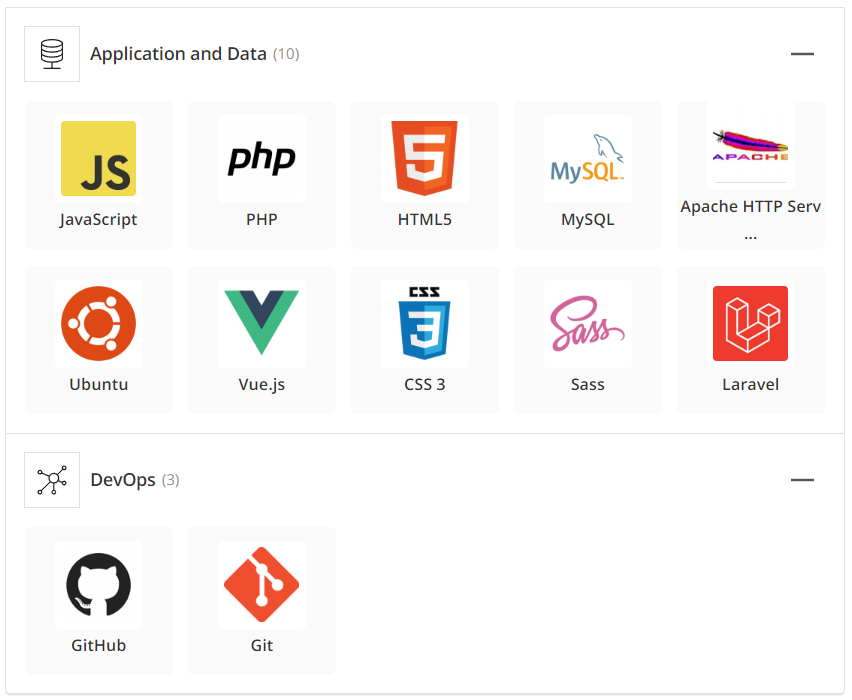
\includegraphics{/assets/figures/stack-old-tb.png}

\subsection{Besoins pour le projet}
Je vais ici définir les besoins du projet et ceci en les séparant par parties distinctes.

\subsubsection{Besoins pour l'infrastructure de développement}
Pour commencer, définissons l'infrastructure de développement.
L'infrastructure de développement englobe tous les outils à installer et toutes les configurations à réaliser sur un pc vierge afin que le développeur puisse commencer à développer l'application.
En général, ce qui est recherché, c'est la simplicité et la rapidité de configuration de cet environnement.
Dans notre cas, pour que le développeur puisse commencer à développer, il doit principalement mettre en place les outils suivants:
\begin{itemize}
    \item un IDE (Integrated Development Environment), de préférence Visual Studio Code,
    \item l'outil de versioning git,
    \item un SGBD (Système de Gestion de Base de Données), %\cite{}
    \item le language PHP,
    \item l'outil Composer,
    \item le framework Laravel,
    \item l'environement d'exécution (runtime environment) Node.js,
    \item le framework Vue.js.
\end{itemize}
Comme vous pouvez le voir, la liste devient vite longue et certains des outils à installer prennent passablement de temps et possèdent des configuration spécifiques.
Je parle notamment des outils suivants:
\begin{itemize}
    \item le SGBD (Système de Gestion de Base de Données),
    \item le language PHP, avec Composer et le framework Laravel,
    \item l'environement d'exécution (runtime environment) Node.js et le framework Vue.js.
\end{itemize}
Ces outils n'étant pas triviaux à mettre en place et changeant pour chaque projet, il est préférable de simplifier le plus possible leur installation et configuration.

Comme vous l'aurez compris, un des besoins le plus important pour le choix de cette infrastructure, est la simplicité de mise en place du projet.
Il faut que cela soit facile à prendre en main et bien documenté.
Un des autres points à prendre en compte, est la disponibilité des outils utilisés, dans le sens où des outils payants ne pourraient pas être accessibles pour certains développeur.
Créer quelque chose de simple à prendre en main, c'est important, mais il faut aussi prendre en compte la difficulté nécessaire pour mettre en place les outils facilitant la prise en main, par exemple Docker.

\subsubsection{Besoins pour l'infrastructure de production}
Nous allons maintenant faire de même pour l'infrastructure de production.
L'infrastructure de production englobe tous les outils à installer et toutes les configurations à réaliser sur un pc vierge afin que le programme final soit accessible est utilisable par n'importe quel utilisateur.
En général, la simplicité de mise à jour du programme, la performance et la robustesse sont recherchés.
On peut aussi prendre en compte la flexibilité de la solution, dans le sens où il serait facile de déployer le programme final sur une autre machine de production.
En effet, la première étape de configuration se réalise peu de fois et si cette dernière est un peu plus compliquée, cela n'est pas forcément un énorme désavantage.
Dans notre cas, pour que le programme puisse fonctionner sur le serveur de production, il est nécessaire d'installer tous les outils suivants:
\begin{itemize}
    \item potentiellement l'outil de versioning git,
    \item un SGBD (Système de Gestion de Base de Données),
    \item le language PHP,
    \item l'outil Composer,
    \item le framework Laravel,
    \item Un serveur Apache,
    \item Un proxy.
\end{itemize}
La liste des outils à installer et configurer, comme pour l'environnement de développement, est conséquente.
Certains outils prennent passablement de temps et possèdent des configuration spécifique.
Je parle notamment des outils suivants:
\begin{itemize}
    \item le SGBD (Système de Gestion de Base de Données),
    \item le language PHP, avec Composer et le framework Laravel.
\end{itemize}
Comme expliqué précédemment, une certaine flexibilité et simplicité est recherchée lors de la mise en place de l'infrastructure et c'est pour cela qu'il est préférable de simplifier le plus possible l'installation et la configuration des outils cités ci-dessus..

Si nous résumons les critères qui influenceront notre décision, nous pouvons ressortir ces derniers:
\begin{itemize}
    \item la performance de l'infrastructure,
    \item la simplicité de mise à jour du programme au sein de l'infrastructure,
    \item la robustesse de l'infrastructure,
    \item la flexibilité de l'infrastructure.
\end{itemize}

\subsubsection{Besoins pour les Devops}
Pour finir, nous allons maintenant faire de même pour le pipeline \Gls{devops}.
Le pipeline \Gls{devops} défini toutes les étapes réalisées et les outils utilisé pour parvenir à mettre en place une infrastructure de travail et de livraison de produit fonctionnel et automatisée au maximum.
Le but des \Gls{devops} étant d'automatisé le plus de tâches possibles, on attend du donc du pipeline les critères suivants:
\begin{itemize}
    \item la performance de l'infrastructure (dans le sens de la rapidité),
    \item la "simplicité" de mise en place du pipeline,
    \item la simplicité de mise à jour du pipeline via une flexibilité maximum,
    \item la robustesse du pipeline,
    \item la possibilité d'ajouter des étapes intermédiaires de tests du produit entre l'infrastructure de développement et de prodution.
\end{itemize}

La flexibilité et simplicité ressort encore une fois dans les besoins de cette section.
Mais un point important est la possibilité de tester manuellement son produit avant de le livrer en production.

\subsubsection{Importance de l'open source et de la gratuité des outils}
Pour tous les choix technologiques qui vont être réaliser, un besoin essentiel intervient.
Plus nous utilisons d'outils open source ou gratuit, plus nous faciliterons l'intégration de n'importe quel développeur au projet, mais pas que.
Utiliser des outils qui sont gratuits ou open source est un plus pour l'intégration aux DevOps car il facilitera de façon non négligeable la mise en place de ces derniers.

% docker
\subsection{Introduction à Docker}
Pour pour pouvoir comparer les différentes infrastructures et faire des choix sur ces dernière, il est important d'introduire l'outil \Gls{docker}.
Docker est un outil permettant de gérer des containers.
Qu'est-ce qu'un container? Un container est une sorte de machine virtuelle plus légère ayant pour but d'encapsuler une ou plusieurs applications / outils technologiques ainsi que toutes les dépendances que ces applications exigent pour leur bon fonctionnement.
Il ne s'agit donc pas de virtualisation mais de "conteneurisation" ou "containerization" en anglais.
Dans une "conteneurisation", seul l'OS et le software est virtualisé et non le hardware.
Nous remarquons bien la différence avec la figure suivante: %\ref{}
%\begin{figure}
%\caption{\href{https://www.docker.com/wp-content/uploads/2021/11/}docker-containerized-and-vm-transparent-bg.png}
%fig{docker-containerized-and-vm.png}{Comparaison entre containeurs docker et machines virtuelles}
%\caption{Comparaison entre conteneurs et machines virtuelles}
%\end{figure}

Les containers sont facilement téléchargeables et transmissibles. Ils sont également relativement facile à mettre en place.
Le principe est simple, nous avons une application et une certaine configuration qui fonctionne, nous pouvons facilement l'encapsuler dans un container et le transmettre à nos collègues ou le télécharger sur un autre pc.
Un des principales avantages, est le fait que le container ne dépend pas de l'OS ou de l'état de la machine sur lequel il va être lancé.
Le seul point requis, est de posséder docker sur la machine.
Cette solution rend plus flexible et portable l'exécution d'application sur n'importe quelle machine.
Voici un schéma démontrant la façon dont docker et des containers dockers sont mis en place sur une machine: %\ref{}
%\begin{figure}
%\caption{Conteneurisation d'applications \href{https://www.docker.com/wp-content/uploads/2021/11/container-what-is-container.png}}
%fig{docker-containerized-and-vm.png}{Comparaison entre containeurs docker et machines virtuelles}
%\end{figure}
%https://www.docker.com/resources/what-container/
%https://www.ibm.com/fr-fr/cloud/learn/docker
%https://fr.wikipedia.org/wiki/Docker_(logiciel)
%https://www.youtube.com/watch?v=Gjnup-PuquQ

Voici une liste des avantages généraux de Docker comparé à une VM:
\begin{itemize}
    \item Les containers sont petits comparé au VM, \cite{koukia}
    \item Les containers utilisent moins de ressources, \cite{koukia}
    \item Les containers démarrent plus rapidement, \cite{koukia}
    \item Fonctionne bien avec les DevOps et les CI/CD, \cite{koukia,data-flair-pros-cons,data-flair-use-cases}
    \item facilite l'extensibilité horizontale. \cite{data-flair-use-cases}
\end{itemize}

Voici une liste des inconvénients de Docker comparé à une VM:
\begin{itemize}
    \item La sécurité, \cite{koukia}
    \item L'isolation non complète', \cite{koukia}
    \item La gestion du réseau. \cite{koukia}
\end{itemize}

% Packaging software in a way that leverages the skills developers already have. \cite{kane2018docker}
% Bundling application software and required OS filesystems together in a single standar‐dized image format. \cite{kane2018docker}
% Using packaged artifacts to test and deliver the exact same artifact to all systems in all environments. \cite{kane2018docker}
% Abstracting software applications from the hardware without sacrificing resources \cite{kane2018docker}

On peut voir ici une liste des cas d'utilisations de docker \cite{data-flair-use-cases}: %\ref{}
% TODO ajouter image docker use cases
%\begin{figure}
%\caption{Cas d'utilisation de docker \href{https://data-flair.training/blogs/wp-content/uploads/sites/2/2018/10/}}
%\fig{docker-use-cases.jpg}{Cas d'utilisation de docker}
%\end{figure}

% quand ne pas utiliser docker: Performance is critical to your application

%virtual machine vs containers:
%https://www.youtube.com/watch?v=cjXI-yxqGTI
%https://www.ibm.com/cloud/learn/containers?utm_medium=OSocial&utm_source=Youtube&utm_content=000023UA&utm_term=10010608&utm_id=YTDescription-101-Containers-vs-VMs-LH-Containers-Guide&cm_mmc=OSocial_Youtube-_-Cloud+and+Data+Platform_SFT+Cloud+Platform+Digital-_-WW_WW-_-YTDescription-101-Containers-vs-VMs-LH-Containers-Guide&cm_mmca1=000023UA&cm_mmca2=10010608
%https://www.ibm.com/cloud/learn/virtual-machines?utm_medium=OSocial&utm_source=Youtube&utm_content=000005UJ&utm_term=10002434&utm_id=YTDescription-101-Containers-vs-VMs-LH-Virtual-Machines-Guide&cm_mmc=OSocial_Youtube-_-Cloud+and+Data+Platform_PLT+Cloud+Platform+F2F-_-WW_WW-_-YTDescription-101-Containers-vs-VMs-LH-Virtual-Machines-Guide&cm_mmca1=000005UJ&cm_mmca2=10002434


\subsubsection{Performances de Docker}
\Gls{docker} est outil qui paraît très pratique, mais qu'en est-il de ses performances?
Pour ceci, nous allons retracer quelques évalutations réalisées lors d'une étude de IBM. Nous allons parcourir ces évalutations via des graphiques, tiré de l'étude, résumants bien les résultats.
Commençant par la latence que peut apporter \Gls{docker}: %\ref{}
%copier coller et dans la légende, source: x ou tiré de: x
%todo ajouter figure
%\begin{figure}
%\caption{Network round-trip latency (µs) \cite{rad2017introduction}}
%\fig{docker-perf-latency.png}{Latence aller-retour du réseau (µs)}
%\end{figure}

On constate que la latence double, mais nous parlons ici de microsecondes, et de 30 microsecondes supplémentaires, ce qui est en soit assez peu pour de petite infrastructure.

En ce qui concerne le transfert de grosses quantité de données via TCP, docker parvient à se rapprocher des performances d'une machine native, elles n'utilisent donc pas beaucoup plus de cycles: %\ref{}
%\begin{figure}
%\caption{TCP bulk transfer efficiency (CPU cycles/byte) \cite{rad2017introduction}}
%\fig{docker-perf-transfer-efficiancy.png}{Efficacité du transfert de masse TCP (cycles CPU/octet)}
%\end{figure}

Au niveau des écritures, on remarque grâce aux deux graphiques suivants que les performances valent celles d'un système natif: %\ref{}
%\begin{figure}
%\caption{Sequential I/O throughput (MB/s) \cite{rad2017introduction}}
%\fig{docker-perf-sequential-io.png}{Débit d'E/S séquentielles (Mo/s)}
%\end{figure}

%\begin{figure}
%\caption{Random I/O throughput (IOPS) \cite{rad2017introduction}}
%\fig{docker-perf-random-io.png}{Débit d'E/S aléatoires (IOPS)}
%\end{figure}

%docker en prod perf:
%https://stackoverflow.com/questions/21691540/how-to-optimize-performance-for-a-docker-container/21707838#21707838
%https://stackoverflow.com/questions/21889053/what-is-the-runtime-performance-cost-of-a-docker-container
%https://dominoweb.draco.res.ibm.com/reports/rc25482.pdf
%https://www.freecodecamp.org/news/7-cases-when-not-to-use-docker/


\subsubsection{Et Kubernetes?}
Pourquoi utiliserions-nous forcément docker sans avoir réfléchi à la possibilité de \Gls{kubernetes}?
Pour commencer, comme indiquer sur le site officiel:
"Kubernetes est un système open-source permettant d'automatiser le déploiement, la mise à l'échelle et la gestion des applications conteneurisées".
Kubernetes n'est donc pas vraiment une alternative à docker, mais peut être plutôt utiliser comme complément à ce dernier.
Comme la partie principale de Kubernetes est de gérer les applications conteneurisées et de simplifier le load balancing, par exemple, il n'est pas forcément utile pour nous d'approfondir les recherches sur le sujet.
En effet, La charge attendu par l'application déployée ne devrait pas dépasser les 100 utilisateurs simultanés. La question du load-balancing est donc écartée, tout comme la mise en place d'un cluster Kubernetes.

% comment mettre en place -> voir avec monsieur Graf / regarder avec des profs
% si question pointu, peuvent être transférer à m. chevallier

%https://kubernetes.io/
%https://www.youtube.com/watch?v=PziYflu8cB8
%docker vs k8s, IBM: https://www.youtube.com/watch?v=2vMEQ5zs1ko
%https://www.ibm.com/cloud/learn/kubernetes?cm_mmc=OSocial_Youtube-_-Hybrid+Cloud_Cloud+Platform+Digital-_-WW_WW-_-KubevsDockerYTDescription&cm_mmca1=000023UA&cm_mmca2=10010608#toc-what-is-ku-nVcfWlWE

%https://stackshare.io/: outil très utile pour faire des comparaisons de technologies

\subsubsection{Autres solutions de containers}
% TODO
Pourquoi utiliserions-nous forcément \Gls{docker}
-> beaucoup moins utilisé

\begin{itemize}
    \item BSD Jails, %https://fr.wikipedia.org/wiki/BSD_Jail
    \item LXD, %https://linuxcontainers.org/lxd/
    \item LXC, %https://linuxcontainers.org/lxc/introduction/
    \item Solaris Zones, %https://docs.oracle.com/cd/E18440_01/doc.111/e18415/chapter_zones.htm#OPCUG426
    \item RKT. %https://www.redhat.com/en/topics/containers/what-is-rkt
\end{itemize}

% dev
\subsection{Infrastructures de développement}

\subsubsection{Présentation des infrastructures de développement possibles}
L'infrastructure que vous pouvez voir dans la figure ci-dessous et celle qui était utilisée lorsque j'ai reprise le projet.
En résumé, tous les outils ont été installés nativement sur la machine de développement sans virtualisation.
\figi{infrastructure-dev-actuelle.drawio}{16cm}{Infrastructure de développement actuelle}

\figi{infrastructure-dev-db-docker.drawio}{16cm}{Infrastructure de développement avec une DB en Docker}

\figi{infrastructure-dev-db-laravel-docker.drawio}{16cm}{Infrastructure de développement avec une DB et Laravel en Docker}

Laravel \href{https://laravel.com/docs/9.x/homestead}{Homestead} est un environnement de développement virtualisé à l'aide d'une machine virtuelle \href{https://www.vagrantup.com/}{Vagrant}.
Cette solution est considérée comme le prédecesseur à Laravel Sail qui est beaucoup plus léger.
C'est pourquoi, cette solution ne fera pas parti des choix que nous allons argumenter, mais est présentée comme complément.
\figi{infrastructure-dev-laravel-homestead.drawio}{16cm}{Infrastructure de développement avec Laravel Homestead}

\figi{infrastructure-dev-db-laravel-vuejs-docker.drawio}{16cm}{Infrastructure de développement avec une DB, Laravel et Vue.js en Docker}

%https://laravel.com/docs/9.x/sail
%https://blog.logrocket.com/laravel-and-docker-a-guide-to-using-laravel-sail/
%https://r00t4bl3.com/post/how-to-setup-docker-environment-for-laravel-development
%https://dockerize.io/guides/php-laravel-guide
%https://www.honeybadger.io/blog/laravel-docker-php/

\clearpage

\subsubsection{Évolutions de l'infrastructure de développement possibles}
Les différentes infrastructures désormais présentées, il est nécessaire de les comparer en listant les pour et les contres de chaque changement en prenant comme référentielle l'infrastructure actuelle.
Les 3 améliorations (combinées ou non) proposées sont les suivantes:
\begin{itemize}
    \item Passage du SGBD en machine Docker,
    \item Passage du projet Laravel (et toutes ces technologies) en machine Docker,
    \item Passage du projet Vue.js (et toutes ces technologies) en machine Docker.
\end{itemize}

\subsubsection{Passage du SGBD en conteneur Docker}
\begin{multicols}{2}[Commençons par réfléchir sur le passage du SGBD en conteneur Docker.]
    % vraiment bien se blinder au niveau des arguments via blog et études, sources écrites
    % si on a pas trouvé, on peut dire je ne sais pas, on DOIT dire -> joker ultime
    % toucher quelque chose en surface, si je ne connais pas, si point essentiel dans projet, faire un choix + essai -> prototype, démonstration sur expérience
    % aussi parlé des charges qui devront être supportées et si c'est possible, nb user final par ex
    Pour ceci, nous allons énumérer les avantages et inconvénients d'installer le SGBD nativement.
    Avantages:
    \begin{itemize}
        \item Gestion de la BD plus facile car le SGB est installé nativement,
        \item Le SGBD peut-être déjà installé et peut être utilisée directement,
        \item Ne nécessite pas Docker.
    \end{itemize}

    Inconvénients:
    \begin{itemize}
        \item Demande du temps pour l'installation,
        \item Configuration à réaliser à la main,
        \item Fort risque d'erreur lors de la configuration,
        \item Installation différente pour chaque OS.
    \end{itemize}

    \columnbreak
    Nous allons, maintenant, énumérer les avantages et inconvénients d'avoir le SGBD en machine Docker.
    Avantages:
    \begin{itemize}
        \item Accélère l'installation de l'environnement de développement, \cite{labrecque,data-flair-pros-cons}
        \item Apporte de la cohérence au niveau des technologies utilisées, au sein de l'équipe, \cite{labrecque, data-flair-use-cases}
        \item Rend le debugging dû aux environnements de développement plus facile, \cite{labrecque,koukia}
        \item Facilite la configuration, car elle est en gande partie déjà réalisée, \cite{data-flair-pros-cons}
        \item Compatible avec tous les OS.
    \end{itemize}

    Inconvénients:
    \begin{itemize}
        \item Gestion de la BD potentiellement plus compliquée,
        \item \Gls{docker} peut avoir des problèmes de performances, \cite{labrecque}
        \item Nécessite Docker et les connaissances qui vont avec. \cite{labrecque}
    \end{itemize}
\end{multicols}

Si nous évaluons les deux solutions proposées selon les besoins suivants:
\begin{itemize}
    \item simplicité de mise en place du projet,
    \item la disponibilité des outils utilisés,
    \item la difficulté nécessaire pour mettre en place les outils facilitant la prise en main.
\end{itemize}

On se rend facilement compte que la solution avec Docker est celle qui se rapproche le plus de ces derniers.

\subsubsection{Passage de Laravel en conteneur Docker}
\begin{multicols}{2}[Passons maintenant au passage de l'environnement Laravel en conteneur Docker.]
    Pour ceci, nous allons énumérer les avantages et inconvénients d'installer nativement cet environnement.
    Avantages:
    \begin{itemize}
        \item (Meilleur performance),
        \item Gestion totale de l'environnement.
    \end{itemize}

    Inconvénients:
    \begin{itemize}
        \item Peut générer des conflits si plusieurs versions sont présentes,
        \item Impossibilité d'avoir plusieurs versions différentes installées,
        \item L'installation demande du temps,
        \item Configuration à faire à la main,
        \item Fort risque d'erreur lors de la configuration,
        \item Installation différente pour chaque OS.
    \end{itemize}

    \columnbreak
    Nous allons, maintenant, énumérer les avantages et inconvénients d'avoir l'environnement Laravel en machine Docker.
    Avantages:
    \begin{itemize}
        \item Accélère l'installation de l'environnement de développement, \cite{labrecque}
        \item Apporte de la cohérence au niveau des technologies utilisées, au sein de l'équipe, \cite{labrecque, data-flair-use-cases}
        \item Rend le debugging dû aux environnements de développement plus facile, \cite{labrecque,koukia}
        \item Facilite la configuration, car elle est en gande partie déjà réalisée, \cite{data-flair-pros-cons}
        \item Compatible avec tous les OS,
        \item Existance d'un outil donné par Laravel et conçu pour être utiliser avec \Gls{docker}, il s'agit de \href{https://laravel.com/docs/9.x/sail}{Sail},
        \item Permet d'avoir plusieurs versions installées.
    \end{itemize}

    Inconvénients:
    \begin{itemize}
        \item \Gls{docker} peut avoir des problèmes de performances, \cite{labrecque}
        \item Nécessite Docker et les connaissances qui vont avec. \cite{labrecque}
    \end{itemize}
\end{multicols}

Si nous évaluons les deux solutions proposées selon les besoins suivants:
\begin{itemize}
    \item simplicité de mise en place du projet,
    \item la disponibilité des outils utilisés,
    \item la difficulté nécessaire pour mettre en place les outils facilitant la prise en main.
\end{itemize}

On se rend facilement compte que la solution avec Laravel Sail est celle qui se rapproche le plus de ces derniers. Et que encore une fois, la solution contenant du Docker paraît assez adaptée.

%https://laravel.com/docs/9.x/sail
%https://laravel.com/docs/9.x/homestead

\subsubsection{Passage de Vue.js en conteneur Docker}
\begin{multicols}{2}[Finalement, parlons du passage de l'environnement Vue.js en conteneur Docker.]
    Pour ceci, nous allons énumérer les avantages et inconvénients d'installer nativement cet environnement.
    Avantages:
    \begin{itemize}
        \item (Meilleur performance),
        \item Node.js possède un bon gestionnaire de version,
        \item Compatible avec tous les OS,
        \item Gestion totale de l'environnement.
    \end{itemize}

    Inconvénients:
    \begin{itemize}
        \item Configuration à faire à la main,
    \end{itemize}

    \columnbreak
    Nous allons, maintenant, énumérer les avantages et inconvénients d'avoir l'environnement Laravel en machine Docker.
    Avantages:
    \begin{itemize}
        \item Rapide à installer,
        \item Configuration en gande partie déjà réalisée,
        \item Compatible avec tous les OS.
    \end{itemize}

    Inconvénients:
    \begin{itemize}
        \item Nécessite Docker et les connaissances qui vont avec,
        \item Peut-être compliqué à mettre en place.
    \end{itemize}
\end{multicols}

Si nous évaluons les deux solutions proposées selon les besoins, désormais bien connus et suivants:
\begin{itemize}
    \item simplicité de mise en place du projet,
    \item la disponibilité des outils utilisés,
    \item la difficulté nécessaire pour mettre en place les outils facilitant la prise en main.
\end{itemize}

On se rend compte que la solution avec Docker n'apporte pas forcément assez d'avanatages comparé à celle proposant l'installation native et cela est principalement dû au bon gestionnaire de paquets NPM de Javascript. C'est pourquoi, solution proposant l'installation native sera préférée.
%https://www.npmjs.com/

\subsubsection{Résultat de l'analyse}
Suite à cette analyse des outils, la solution la plus adaptée semble être de mettre en place l'environement de développment suivant:

\begin{table}[h]
    \begin{center}
        \caption{Environement de développment choisi \label{env_dev}}
        \begin{tabular}{c|l|r}
            Outil             & Technologie utilisée  \\ \hline
            SGBD - MySQL      & Docker                \\
            Frontend - Vue.js & Installation native   \\
            Backend - Laravel & Laravel Sail (Docker) \\
        \end{tabular}
    \end{center}
\end{table}


Finalement cela correspond à la figure numéro %TODO \href{}{}.

% prod
\clearpage
\subsection{Infrastructures de production}

\subsubsection{Présentation des infrastructures de production possibles}
L'infrastructure de production que vous pouvez voir dans la figure ci-dessous et celle qui était utilisée lorsque j'ai reprise le projet.
En résumé, tous les outils ont été installés nativement sur la machine de développement sans virtualisation.
\figi{infrastructure-prod-actuelle.drawio}{16cm}{Infrastructure de production actuelle}

Cette figure-ci, montre la première amélioration possible, c'est à dire, de passer le SGBD en container docker.
\figi{infrastructure-prod-db-docker.drawio}{16cm}{Infrastructure de production avec une db en docker}

Cette figure-ci, montre la secondes amélioration possible (mais aussi la première), c'est à dire, de passer l'application web réalisée avec le framework Laravel en container docker.
\figi{infrastructure-prod-db-laravel-docker.drawio}{16cm}{Infrastructure de production avec une db et laravel en docker}

\subsubsection{Évolutions de l'infrastructure de production possibles}
Les différentes infrastructures possibles désormais présentées, il est nécessaire de les comparer en listant les pour et les contres de chaque changement en prenant comme référentielle l'infrastructure actuelle.
Les deux améliorations (combinées ou non) proposées sont les suivantes:
\begin{itemize}
    \item Passage du SGBD en machine Docker,
    \item Passage du projet Laravel (et toutes ces technologies) en machine Docker.
\end{itemize}

\subsubsection{Passage du SGBD en conteneur Docker}
\begin{multicols}{2}[Nous recommençons également par réfléchir sur le passage du SGBD en machine Docker.]
    Pour ceci, nous allons énumérer les avantages et inconvénients d'installer le SGBD nativement.
    Certains peuvent être les mêmes qu'énumérer dans la partie "Infrastructure de développement". %\href TODO
    Avantages:
    \begin{itemize}
        \item Gestion de la BD plus facile car le SGB est installé nativement,
        \item Sauvegarde aisément réalisable,
        \item Mise en place d'un service de façon trivialle,
        \item Le SGBD peut-être déjà installé et peut être utilisée directement,
        \item Ne nécessite pas Docker.
    \end{itemize}

    Inconvénients:
    \begin{itemize}
        \item Demande du temps pour l'installation,
        \item Configuration à réaliser à la main,
        \item Fort risque d'erreur lors de la configuration,
        \item Installation différente pour chaque OS.
    \end{itemize}

    \columnbreak
    Nous allons, maintenant, énumérer les avantages et inconvénients d'avoir le SGBD en machine Docker.
    Avantages:
    \begin{itemize}
        \item Accélère l'installation de l'environnement de production,
        \item Facilite la mise à jour de l'environnement de production si l'environnement de développement intègre un containeur docker pour le SGBD,
        \item Configuration en gande partie déjà réalisée,
        \item Compatible avec tous les OS.
    \end{itemize}

    Inconvénients:
    \begin{itemize}
        \item Gestion de la BD potentiellement plus compliquée,
        \item Sauvegarde de la BD potentiellement plus compliquée,
        \item Mise en place d'un service non trivial,
        \item \Gls{docker} peut avoir des problèmes de performances, \cite{labrecque}
        \item Nécessite Docker et les connaissances qui vont avec. \cite{labrecque}
    \end{itemize}
\end{multicols}
% TODO reciter besoins et dire solution qui se rapproche le plus

\subsubsection{Passage de Laravel en conteneur Docker}
\begin{multicols}{2}[Passons maintenant au passage de l'environnement Laravel en conteneur Docker.]
    Pour ceci, nous allons énumérer les avantages et inconvénients d'installer nativement cet environnement.
    Avantages:
    \begin{itemize}
        \item (Meilleur performance),
        \item Gestion totale de l'environnement.
    \end{itemize}

    Inconvénients:
    \begin{itemize}
        \item Mise à jour compliquée si un changement de version à lieu,
        \item L'installation demande du temps,
        \item Configuration à faire à la main,
        \item Fort risque d'erreur lors de la configuration,
        \item Installation différente pour chaque OS.
    \end{itemize}

    \columnbreak
    Nous allons, maintenant, énumérer les avantages et inconvénients d'avoir l'environnement Laravel en machine Docker.
    Avantages:
    \begin{itemize}
        \item Mise à jour du programme facilitée, dans tous les cas,
        \item Accélère l'installation de l'environnement de production,
        \item Configuration en gande partie déjà réalisée,
        \item Offre une possibilité d'extensibilité horizontale,
        \item Compatible avec tous les OS.
    \end{itemize}

    Inconvénients:
    \begin{itemize}
        \item Peut laisser des failles de sécurité, suivant l'environnement mis en place,
        \item Docker peut avoir des problèmes de performances, \cite{labrecque}
        \item Nécessite Docker et les connaissances qui vont avec. \cite{labrecque}
    \end{itemize}
\end{multicols}

% TODO reciter besoins et dire solution qui se rapproche le plus

% TODO pour le déploiment, regarder pourquoi certains sont parti de docker


Suite à cette analyse des outils, la solution la plus adaptée semble être de mettre en place l'environement de développment suivant:

\begin{table}[h]
    \begin{center}
        \caption{Environement de développment choisi \label{env_prod}}
        \begin{tabular}{c|l|r}
            Outil             & Technologie utilisée \\ \hline
            SGBD - MySQL      & Docker               \\
            Backend - Laravel & Docker               \\
        \end{tabular}
    \end{center}
\end{table}

\subsubsection{Analyse de risques}
% comment protéger une infra en prod
% contacter des profs de sécu
% lister ce qu'on va mettre en place
% on est resté en surface, il faudrait investir des experts pour évaluer. (audit par exemple)
% sécurité pas prise en compte dans le projet car pas dans objectif, pas le luxe de rechercher car trop de temps, à mentionner dans le rapport.

L'analyse de risques de l'infrastructure de production est point très important lorsque que l'on publie un logiciel. Cette dernière peut être très complexe et nécessite énormément de connaissances.
Une analyse de risque complète demande une quantité conséquent de travail. L'intervention d'expert dans le domaine, via par exemple, des audits serait une solution pour réaliser cette partie du projet. \newline
L'analyse de risques ne pourra donc pas être réaliser lors de ce projet, pour toutes les raisons énumérées plus haut, mais aussi car ce n'est pas le but principal de ce dernier.
J'ai donc décider d'appliquer tout ce que je connaissais et faire le meilleur travail possible sans aller en profondeur dans le sujet.

% devops
%https://blog.logrocket.com/how-to-create-a-ci-cd-for-a-laravel-application-using-github-actions/

\clearpage
\subsection{Pipeline DevOps}
\subsubsection{Introduction aux Devops}
%https://www.youtube.com/watch?v=scEDHsr3APg
%https://www.padok.fr/blog/devops-tout-savoir
%https://azure.microsoft.com/en-us/overview/what-is-devops/#devops-overview
%https://www.ibm.com/cloud/learn/devops-a-complete-guide
Pour commencer, c'est quoi les DevOps?
Les DevOps c'est un ensemble de processus qui permettent de gérer et faciliter le développement et le déploiement continu de l'application. Cela permet de garantir une meilleur qualité du code et de simplifier l'intégration de ce dernier. C'est-à-dire, si un collaborateur souhaite ajouter sa partie du code au projet, il doit d'abord passer par un système automatisé de contrôle et d'intégration de son code avant de pouvoir l'ajouter. Cette partie est appelée \Gls{ci}.
Les DevOps intègre également tout ce qui est déployement continu et livraison continue (\Gls{cd}).
En pratique, ils intègrent également d'autre aspect, comme la maintenance de l'infrastructure de production et développement, la sécurité des processus et beaucoup d'autres concepts.
Au final c'est un cycle de vie visant à faciliter le développement d'applications en équipe.
Ci-dessous, on peut observer un exemple de lifecycle fourni par IBM:
%\begin{figure}
%\caption{Cycle de vie de développement - IBM}
%\fig{ibm-devops-lifecycle.png}{Cycle de vie de développement - IBM}
%\end{figure}


Aucun Devops ou pipeline n'avait été réalisé lors du précédent projet.
Nous avons donc que des propositions, sans solution existante (ce qui était le cas pour d'autres choix).
Avant de présenter chacun des pipeline DevOps proposé, il est nécessaire d'expliquer pourquoi chacun de ces derniers passent par Github, et plus précisément, les Github Actions.

\subsubsection{Pourquoi Github?}
Tout d'abord, il faut comprendre qu'il existe d'autres outil de "gestion" de \Gls{devops}, appelé aussi services de \Gls{ci} / \Gls{devops}, en voici une liste non exhaustive:
\begin{itemize}
    \item Jenkins \href{https://www.jenkins.io/},
    \item TeamCity \href{https://www.jetbrains.com/teamcity/},
    \item CircleCI \href{https://www.guru99.com/top-20-continuous-integration-tools.html},
    \item Travis-CI \href{https://www.travis-ci.com/},
    \item GitLab \href{https://about.gitlab.com/},
    \item Bamboo \href{https://www.atlassian.com/software/bamboo},
    \item GoCD \href{https://www.gocd.org/},
    \item Azure DevOps \href{https://azure.microsoft.com/fr-fr/services/devops/}.
\end{itemize}

Tous ces outils, mise à part GitLab, doivent être installé en plus et configurer pour le projet.
Comme il s'agit d'un projet assez restreint et n'impliquant que peu de personnes, nous cherchons à rester dans une solution simple et donc "all in one".
Nous n'allons donc pas plonger dans les détails de chaque technologie citée plus haut.
Parmi les solutions "all in one", c'est-à-dire qui propose des services de \Gls{ci} / \Gls{devops} et permette le versioning de code, il reste uniquement GitLab et Github comme choix.
Ne souhaitant pas réaliser une profonde analyse sur ces 2 solutions, car les 2 étant souvent considérées comme équivalentes ou interchangeable, ma connaissance de la solution Github est un argument suffisant, selon moi, pour faire pencher la balance en sa faveur.
% Tous les outils CI / CD
%https://katalon.com/resources-center/blog/ci-cd-tools#
%https://www.lambdatest.com/blog/31-best-ci-cd-tools/
%https://www.guru99.com/top-20-continuous-integration-tools.html
%https://stackshare.io/stackups/github-actions-vs-gitlab-ci#pros

\subsubsection{Présentation des pipeline Devops possibles}
Ce premier pipeline possible possède uniquement un intérêt si l'infrastructure de production tourne à l'aide de conteneurs Docker. En effet, le but est de construire l' /les image(s) Docker contenant tout ce qui est nécessaire (configurations, programmes, etc.) au niveau de la machine de développement, puis d'envoyer cette / ces dernière(s) sur un repository d'image, en l'occurence, Dockerhub. Puis de récupérer cette / ces images sur la machine de production et les lancer simplement.
\figi{devops-dockerhub.drawio}{16cm}{DevOps via dockerhub}

Ce second pipeline, passerait par une plateforme appelée Heroku. Heroku permet de déployer son application sur l'un de leur serveur, puis le redéployer sur une machine de production finale.
Cette approche est très intéressante car l'étape intermédiaire permet de tester l'application sur une autre machine que celle de développement et ceci avant de livrer en production.
\figi{devops-heroku.drawio}{16cm}{DevOps via heroku}
%https://devcenter.heroku.com/articles/getting-started-with-laravel

Finalement, le pipeline passant uniquement par Github, est la solution la plus simpliste en terme du nombre de technologies utilisées. Cette dernière repose sur le fait de simplement pousser le code sur Github et de le mettre à jour sur la machine de production via un script qui récupère les données sur le Github.
\figi{devops-github.drawio}{16cm}{DevOps via github}

\subsubsection{Comparaison des pipeline Devops possibles}
Nous allons définir pour chacun des pipeline, les avantages et inconvénients de ces derniers.
Mais pour réaliser cette section, certains prototypes doivent être réalisés, ainsi que des recherches appronfidie sur la mise en oeuvre des différents pipeline.
En effet, n'étant pas expert dans le domaine, et n'ayant pas le temps de le devenir le temps de ce travail, l'un des critères / besoins importants et la facilité de mise ne place du pipeline.

% pipeline docker
Commençons par le pipeline Docker:
\begin{itemize}
    \item x
\end{itemize}

Inconvénients:
\begin{itemize}
    \item x
\end{itemize}

Continuons avec le pipeline Heroku:
\begin{itemize}
    \item x
\end{itemize}

Inconvénients:
\begin{itemize}
    \item x
\end{itemize}

Finissons avec le pipeline Github:
\begin{itemize}
    \item x
\end{itemize}

Inconvénients:
\begin{itemize}
    \item x
\end{itemize}

% TODO reciter besoins et dire solution qui se rapproche le plus

%\clearpage
%\subsection{Système de gestion de base de données}
% postgre vs mysql
%https://www.geeksforgeeks.org/difference-between-mysql-and-postgresql/
%https://www.simplilearn.com/tutorials/sql-tutorial/postgresql-vs-mysql
%https://www.ibm.com/cloud/blog/postgresql-vs-mysql-whats-the-difference
%https://stackshare.io/stackups/mysql-vs-postgresql

% upgrade to laravel 9
%https://laravel.com/docs/9.x/upgrade
%https://github.com/laravel/vonage-notification-channel/blob/3.x/UPGRADE.md

%\begin{figure}
%\caption{Stack de technologies utilisées via \href{https://stackshare.io/alecberney/bachelors-thesis}{stackshare}}
%\fig{stack-tb.png}{Stack de technologies utilisées}
%\end{figure}

\chapter{Conception et Réalisation de la BD}
%todo à rendre aussi pour le premier rendu
%todo MLD
%todo model de l'ORM

% TODO before 12.05.2022

Dans toutes les desciptions suivantes, les tirets du bas seront remplacé par des "-" à cause d'un problème de LaTex.

\section{Modèle EA}
Le modèle Entité-Associations est la première étape lors de la conception d'une base de données. Il se rapproche également d'un diagramme de classe classique utiliser pour la POO (programmation orienté objet). \newline
Nous allons décrire chacune des entités et ses relations. \newline
Mais avons ça, voici une légende:\newline
Un rectangle représente une entité et possède son nom dans sa partie supérieur.\newline
Les valeurs textuelles en dessous sont les champs de l'entité. Le champ souligné représente la clé primaire de l'entité, cette dernière doit être unique.\newline
Les traits tiré entre deux entités sont des associations et peuvent se lire dans les deux sens. Les verbes écrits au dessus des traits servent à donner un sens à l'association. \newline
Les symboles et numéros à chaque extrémités des entités indiquent respectivement:
\begin{itemize}
    \item 0 : zéro / aucun,
    \item 1 : un,
    \item 1..* : un ou plusieurs,
    \item * : zéro ou plusieurs.
\end{itemize}

Par exemple, on peut lire l'association "user" - "message", comme ceci: \newline
Un utilisateur peut envoyer zéro ou plusieurs messages. \newline
Un message peut être envoyé que par un utilisateur.

Finalement, certains peuvent être ajouté avec des rectangles pliés en haut à droite et relié avec des traits pointillés.

\figi{ea}{16cm}{Modèle Entitié - Associations de la base de données}

\subsection{Entité user}
L'entité "user" représente un utilisateur de l'application, que ce soit un élève, un professeur ou un technicien.\newline
Il possède des informations classiques le concernant, ainsi que le champ "switch-uuid" représentant l'identifiant unique fourni par le service Switch edu-id qui sera utilisé.\newline
Les champs contenant le mot "notify" servent à stocker les préférences de l'utilisateur concernant les notifications de l'application.

On voit au niveau des relations, que l'utilisateur peut envoyer et recevoir des messages.\newline
Il peut posséder également plusieurs rôles mais doit en posséder au moins un, celui par défaut qui est le rôle "client".\newline
L'utilisateur peut de toute façon faire une demande de travail (job). Cependant, seul les utilisateurs possédant le rôle "validator", en général, les professeurs pourront valider le travail.\newline
Le travail validé, un "worker", en général un technicien, pourra réaliser le travail demander et en indiquer le suivi.

\subsection{Entité job}
L'entité "job" représente un travail demandé par un utilisateur de l'application.\newline
Il possède un id (identifiant unique), une description du travail à réaliser, une date butoir (deadline), une évaluation que l'utilisateur / client peut attribuer au travail terminé et un status d'avancement du travail mis à jour par le travailleur.\newline
Le status d'avancement d'un travail sera défini par un enum (liste exhaustive de valeurs), la voici:
\begin{itemize}
    \item new,
    \item validated,
    \item assigned,
    \item ongoing,
    \item on-hold,
    \item completed.
\end{itemize}

On voit au niveau des relations, que le travail peut posséder des messages qui lui sont liés.\newline
Il posséde également une catégorie de travail définissant ensuite quelles machines peuvent être utilisées pour le réaliser.\newline
Le travail possédera également un utilisateur client, un validateur et un travailleur.\newline
Il doit également contenir un ou plusieurs fichiers nécessaires pour réaliser le travail demandé.\newline
Finalement, certains événements peuvent être lié au travail. On parle ici d'événement permettant de préfevenir l'utilisateur via des notifications ou email.

\subsection{Entité role}
L'entité "role" représente simplement un rôle que peut avoir un utilisateur au sein de l'application. Cette entité est nécessaire car un utilisateur peut posséder plusieurs rôles et ils doivent tous être défini la même chose.\newline
Seul un id (identifiant unique) et un nom du rôle est nécessaire.\newline
Voici la liste des rôles définis:
\begin{itemize}
    \item admin,
    \item client,
    \item worker,
    \item validator.
\end{itemize}

\subsection{Entité message}
L'entité "message" représente un message envoyé entre deux utilisateurs au sujet d'un travail demandé.\newline
Il possède uniquement un id (identifiant unique) et un text.\newline
Il est associé à deux utilisateurs, un représentant celui qui a envoyé le message et l'autre celui qu'il l'a reçu. Le message est également associé au travail dont il est le sujet.\newline
Une aggrégation a été modélisé pour cette dernière association car on souhaite supprimé tous les messages liés à un travail, si ce dernier est supprimé.

\subsection{Entité job-category}
L'entité "job-category" représente une catégorie de travail pouvant être effecutée au fablab, pare exemple, une impression 3D ou une découpe laser.\newline
La catégorie possède un id (identifiant unique), un acronyme et un nom.\newline
Elle est associé à un travail car ce dernier est obligé d'avoir une catégorie.\newline
Elle possède également une ou plusieurs machines (device) sur lesquels peuvent être réaliser les travaux.\newline
Comme elle possède des machines, une liste de type de fichiers acceptés est nécessaire et est défini par l'association "job-category" - "file-type". Cela permettra de facilement vérifier si un fichier donné pour un travail peut être accepté pour la catégorie de ce dernier.

\subsection{Entité device}
L'entité "device" représente une machine / un outil utilisé pour réaliser un travail du fablab.\newline
La machine possède un id (identifiant unique), un nom, une description plus précise et un chemin de fichier où est stocké son image (cette partie pourrait changer).\newline
Comme expliqué précédement dans la catégorie, elle possède une ou plusieurs catégories sur lesquels elle peut être utilisée.\newline

\subsection{Entité file-type}
L'entité "file-type" représente un type de fichier que peut accepter une catégorie de travail du fablab.\newline
Le type de fichier possède un id (identifiant unique), un nom et un mime-type \href{https://developer.mozilla.org/fr/docs/Web/HTTP/Basics_of_HTTP/MIME_Types} étant utiliser pour valider les fichiers télécharger.\newline
Comme expliqué précédement dans la catégorie, un type de fichier possède une ou plusieurs catégories qui sont acceptées.\newline
Le type de fichier peut également être associé à plusieurs fichiers.

\subsection{Entité file}
L'entité "file" représente un fichier fourni pour réaliser un travail du fablab.\newline
Le fichier possède un id (identifiant unique), un nom et un hash de son contenu.\newline
Il est associé à un type de fichier (file-type), ce qui est utile pour faire le lien avec la catégorie du travail.\newline
Il possède évidemment un travail pour indiquer pour auquel il appartient.\newline
Une aggrégation a été modélisé pour cette dernière association car on souhaite supprimé tous les fichiers liés à un travail, si ce dernier est supprimé.

\subsection{Entité event}
L'entité "event" représente un événement concernant un travail du fablab. Par exemple, un événement est généré si le status d'un travail a été modifié ou si un fichier a été ajouté.\newline
L'événement possède un id (identifiant unique) et des données (data).\newline
Il est associé à un travail comme expliqué plus précédement.\newline
Une aggrégation a été modélisé pour cette dernière association car on souhaite supprimé tous les événements liés à un travail, si ce dernier est supprimé.

\subsection{Entité tasks-queue et failed-tasks}
Ces entités ont été modélisées pour effectuer les tâches en arrière plan du backend, comme l'envoi d'email retardé. Elle ne sont pas encore très développée par manque de connaissances de leur fonctionnement.

\section{MLD}
Le modèle logique des données n'est rien d'autre qu'une évolution du modèle EA.\newline
Les entités deviennent des tables et les associations des relations, ce qui est presque la même chose.\newline
Les tables ont pris un nom au pluriel pour respecter la philosophie de Laravel et de son ORM Eloquent.\newline
Les champs obtiennent des types représentant la façon dont ils seront stockés.\newline
Les clés étrangère issues des association s'ajoutent aux tables.\newline
Les associations N à N du modèle EA voient naître une table intermédiaire. Voici celles qui ont été créées:
\begin{itemize}
    \item device-job-category,
    \item file-type-job-category,
    \item role-user.
\end{itemize}

\figi{mld}{16cm}{Modèle logique des données de la base de données}

Sur le schéma, quelques nouveaux symboles apparaîssent, voici une légende:
\begin{itemize}
    \item Clé jaune : clé primaire de la ligne,
    \item Losange bleu : la colonne ne peut pas valoir null,
    \item Losange vide : la colonne peut valoir null,
    \item Losange rouge : la colonne possède une clé étrangère.
\end{itemize}

Une clé étrangère étant le champ représantant une autre table dont une relation existe. La clé primaire représente la table en elle-même, elle est son identifiant.

\subsection{Champs spéciaux}
Quelques champs obtiennet des valeurs précises et méritent une explication.\newline
Les champs switch-uuid et email, de la table "users" possèdent 320 charactères car ils sont tous des emails ou des dérivés et une email peut contenir au maximum 320 charactères.

Le champ status de la table "job" est une enum comme expliqué précédement dans le modèle EA.

\subsection{Remarques}
% TODO
Tous les autres champs n'ont pas encore fait l'objet de recherches ou de spécifications et ont donc souvent une valeur de 45 ou 50 charactères. Cela cera réalisé prochainement.

Les entités concernant les tâches en arrière plan n'apparaîssent pas car elle ne sont pas encore assez connue.

%Certaines colonnes sont communes à plusieurs des tables. C'est le cas de 'created_at',
%qui indique l'heure de création de la ligne, et 'updated_at', qui indique l’heure à
%laquelle la ligne à été modifiée pour la dernière fois.


\section{Migrations Laravel}

Les migrations du backend réalisées avec Laravel et l'ORM Eloquent se rapprochent le plus possibles du MLD présenté précédement.

% TODO: insert code migrations

\subsection{Champs possiblement nulles}

\subsection{Champs timestamps}

\subsection{Clés étrangères}

\subsection{Options de suppression}

\subsection{Indexes}

\chapter{Conception et Réalisation du Backend / de l'API}
%todo à rendre aussi pour le premier rendu
%todo architecture de code
\section{Architectures de code}

\figi{architecture-code-spring.drawio}{16cm}{Architecture de code du framework Spring "classique"}

\figi{architecture-code-laravel.drawio}{16cm}{Architecture de code du framework Laravel "classique"}

\figi{architecture-code-laravel-proposee.drawio}{16cm}{Architecture de code Laravel proposée}

% ensuite décrire ce qu'on a mis en place et indiquer s'il y a des failles

% surtout indiquer tout ce qu'on a fait et tout ce que j'ai pas fait
% et pourquoi je l'ai pas fait, pas compris qqch ou pas eu le temps, pas la priorité, pas de sources suffisantes

%dans le texte (Labrecque, 2018)
%\cite{labrecque}

%suivantes:
%(Labrecque, 2018; x, yyyy;)
%pour reformuler

%Labrecque M. (2018). Pros and cons of Docker. in \textit{Docker, planet drupal}. consulté à %l'adresse: https://affinitybridge.com/blog/pros-and-cons-docker (consulté le 31.03.2022)

\chapter{Intégration continu}

%php unit

\chapter{Déploiement continu}

\chapter{Reprise du projet}

\section{Récupération du physique du projet}

\section{Erreurs restantes}

\section{Améliorations possibles}

%%if
\chapter{Bibliographie}
\section{Citations et bibliographie}
%Citer vos sources est essentiel. Avec \texttt{biblatex} vous pouvez facilement citer des articles, des livres ou des sites internet. Toutes les citations dans le texte seront automatiquement regroupées en fin de document dans la section \guillemotleft Bibliographie\guillemotright. Par exemple, citons un article d'Einstein \cite{einstein} ou le livre de Dirac \cite{dirac}.

Parfois il peut être utile d'utiliser un gestionnaire de bibliographie. La communauté académique recommande l'outil \href{https://www.zotero.org/}{Zotero} qui permet de gérer une bibliothèque numérique d'ouvrages et de références numériques. Il permet également de générer une bibliographie compatible avec \LaTeX.


\mintinline{latex}{\SI{42.12}{\kilo\gram\metre\per\square\second}}\par
%%fi

\chapter{Conclusion}

%%if
Bien que non nécessaire dans un rapport de Bachelor, la discussion finale d'un projet résume les résultats obtenus et dresse une conclusion objective du projet. Un manager de société est souvent amené à lire de nombreux rapport, il ne s'intéresse généralement qu'à l'introduction au contexte de l'étude et à sa conclusion.

Il est de coutume de signer la conclusion...
%%fi

\vfil
\hspace{8cm}\makeatletter\@author\makeatother\par
\hspace{8cm}\begin{minipage}{5cm}
    %%if
    % Place pour signature numérique
    \printsignature
    %%fi
\end{minipage}
\clearpage

\appendix
\appendixpage
\addappheadtotoc

%%if
\chapter{Première annexe}

Les annexes n'ont pas un contenu \underline{normatif} mais \underline{descriptif}. Tout contenu annexé ne doit pas être nécessaire à la bonne compréhension du travail.

Les annexes contiennent généralement :

\begin{itemize}
    \item les dessins mécaniques (mises en plan);
    \item les schémas électriques détaillés;
    \item des photographies du projet;
    \item des scripts et des extraits de code source;
    \item des documents techniques \pex \emph{datasheet};
    \item des développements mathématiques.
\end{itemize}
\section{Sous section}
\lipsum[1]
%%fi

\let\cleardoublepage\clearpage
\backmatter

\label{glossaire}
\printnoidxglossary
\printbibliography
\label{index}
\printindex

\end{document}
